%El objetivo de este documento es identificar, detallar y documentar los casos de uso de nuestra aplicación a partir de la SRS. Esto incluye una narracion
%que describe la secuencia de pasos que  un actor (un agente externo, que no tiene por que ser una persona, es un rol) realiza con el sistema para completar un proceso.
%El tema de casos de uso de IS es el TEMA 3


\documentclass[spanish,a4paper,12pt]{report}	% Idioma, tamaño del papel, tamaño letra, documento (book, report, article, letter)

%%% PAQUETES
\usepackage[spanish,activeacute]{babel}				
% Babel: Adapta cosas como la tipografia, la fecha, lo de Chapter al español, y activeacute para apóstrofes (') como abreviaciones de acentos: \'{a}
\usepackage[utf8]{inputenc}					% Codificacion UTF8 (para meter tildes normal: á --> \'{a} )
\usepackage{multicol}						% Escritura en varias columnas
\usepackage{graphics}						% Inclusión de imágenes
\usepackage{graphicx}						% Mas para imagenes
\usepackage{geometry}						% Distribucion de la pagina: margenes, encabezados, tamaño pagina...
\usepackage{fancyhdr}						% Paquete para añadir y modificar encabezados y pies de pagina
\usepackage{hyperref}						% Para hipervínculos, en el indice al menos, GRACIAS A DAVID
%\usepackage{lastpage}						% Ultima pagina para poner, por ejemplo, 3 de 15
%%% PAQUETES MATEMATICOS
\usepackage{amsmath}						% Conjunto de paquetes desarrollados por la Amercian Matematical Society
\usepackage{amssymb}						% Tipografía mathbb y otros símbolos tambien de la AMS
\usepackage{amsthm}						% Paquete AMS theorem, de la AMS
\usepackage{amsfonts}						% Paquete con símbolos y mas, de la AMS
%\usepackage{nicefrac}						% Fracciones bonitas, LO DEJO COMENTADO PORQUE A VECES DA PROBLEMAS AL COMPILAR


%%% DECLARACIONES (sobre la forma de la pagina, encabezado etc.)
\pagenumbering{roman}						
% Para numerar las paginas en numeros romanos hasta que empiece el texto (tambien alph, Alph, roman, Roman...)
\pagestyle{fancy}							% Utiliza el paquete fancyhdr para encabezados y pies de pagina
%\thispagestyle{empty}  						% Para poner UNA pagina sin encabezados ni numero, "plain" CON numero, "fancy" normal
%\lhead{Encabezado a la izquierda}				% Encabezado a la izquierda
\rhead{\bfseries Casos de uso}				%Encabezado a la derecha
\cfoot{\thepage}							% Numero de pagina centrado en el pie
%\cfoot{\thepage\ de \pageref{LastPage}}		% Numero de pagina centrado en el pie asi: n de m
\renewcommand{\headrulewidth}{0.4pt}			% Linea debajo del encabezado
\renewcommand{\footrulewidth}{0.4pt}			% Linea encima del pie de pagina
\renewcommand*{\thesection}{\arabic{section}}	% Hace que no apareca el indice de capitulos y que comience en section, GRACIAS A RUBEN


%%%%% CUERPO %%%%%
\begin{document}

\title{\textbf{\huge{Documento de \\ 
	casos de uso}} \\ \vspace{0.3cm}
	\Large{Ingeniería del Software}}
\author{ Jesús Aguirre Pemán \\
	 Enrique Ballesteros Horcajo \\
	 Jaime Dan Porras Rhee \\
	 Ignacio Iker Prado Rujas \\
	 Alejandro Villarín Prieto }
\date{\Today}
\maketitle

\newpage
\mbox{}
\thispagestyle{empty}						% Hoja en blanco, sin numeros ni nada
\newpage


\tableofcontents 							%INDICE hipervinvulado

\newpage
\mbox{}
\thispagestyle{empty}						% Hoja en blanco, sin numeros ni nada
\newpage

\pagenumbering{arabic}						% Pone el contador de paginas a 1 y ahora en numeros normales

\part{Extracto} %%% PARTE 1: EXTRACTO %%%______________________________________________________________________________________________
En nuestro proyecto trataremos de desarrollar una aplicación software (y su correspondiente documentación) de la administración de un negocio de hostelería. Se tratará de un Hotel con Restaurante- Bar. La aplicación recogerá toda la información necesaria para el desarrollo próspero de dicho negocio, ésto es, existencias de los productos, gastos de todo tipo, base de datos con los clientes, generación de las cuentas a cobrar, reservas de los clientes, habitaciones disponibles/ ocupadas, mobiliario del que se dispone, balances económicos (accesible sólo al administrador)... Es importante también centrarse en el entorno de la empresa: pequeña, mediana, gran empresa; situación geográfica (no es lo mismo que se emplace en una gran ciudad o en mitad de los Pirineos); gama de productos que se ofrecen (cocina mediterránea, vasca, italiana, china...); tamaño del local... \\

En primer lugar, debemos identificar el problema a solventar, dar su descripción y un minucioso análisis. El problema es idear un software que facilite a sus usuarios el trabajo descrito arriba. Para ello, debe ser sencillo e intuitivo a la vez que seguro y adaptado a los intereses de la empresa que lo solicita. Además hay que centrarse en describir detalladamente las funcionalidades que tendrá. Una vez completa la especificación del sistema, se puede abordar la implementación. Es fundamental que la especificación sea clara y sobre todo precisa, ha de responder a cualquier pregunta sobre su uso y diseño. Una vez terminado, debe someterse a las pruebas correspondientes y a la más importante: ¿el usuario queda satisfecho con los resultados?, ¿la aplicación hace lo que él espera que haga y como él espera que lo haga? Tras esto, con toda seguridad habrá una tarea de mantenimiento, solventando errores que surjan, hasta que, eventualmente, el programa caiga en desuso (obsolescencia).

\newpage
\mbox{}
\thispagestyle{empty}						% Hoja en blanco, sin numeros ni nada
\newpage

\setcounter{section}{0}

\part{Catálogo de casos de uso} %%% PARTE 2: CATALOGO CASOS DE USO %%%____________________________________________________________
En esta primera parte, simplemente enumeramos los casos de uso, clasificándolos en primarios y secundarios, para tener una visión general de los mismos.
\section{Primarios} 				%Los procesos principales, que sean mas comunes de realizar
	\begin{itemize}
%%	INSERTAR ORDENADAMENTE LOS CASOS DE USO, MÁS O MENOS COMO ESTÁN EN EL DOCUMENTO LISTA DE TODOS LOS CASOS DE USO (BRAINSTORMING PARA JESÚS)
%%	HAY QUE TENER EN CUENTA QUE DESPUÉS HAY QUE PONERLOS ABAJO EN EL MISMO ORDEN
	\item \textbf{Login}	
	\item \textbf{Gestionar Empleados}	
	\item \textbf{Acceder a la ficha de un empleado}
	\item \textbf{Añadir cliente}
	\item \textbf{Ver ficha de cliente}
	\item \textbf{Editar cliente}
	\item \textbf{Dar de baja cliente}
	\item \textbf{Organizar tareas de la limpieza}
	\item \textbf{Revisión de limpieza}
	\item \textbf{Consultar tareas}
	\item \textbf{Confirmar limpieza de habitación}
	\item \textbf{Informar de incidencias}	
	\item \textbf{Consultar tareas de  mantenimiento}
	\item \textbf{Reservar mesa}
	\item \textbf{Anular reserva}
	\item \textbf{Generar un pedido para una mesa}
	\item \textbf{Modificar un pedido}
	\item \textbf{Cancelar un pedido}
	\item \textbf{Generar factura a un cliente}
	\item \textbf{Ver menú}
	\item \textbf{Añadir nota}
	\item \textbf{Borrar nota}
	\item \textbf{Ver cuenta diaria de la caja de recepción}
	\item \textbf{Ver cuenta diaria de la caja del restaurante}
	\item \textbf{Consultar libro diario}
	\item \textbf{Consultar libro mayor}
	\item \textbf{Ver habitaciones}	
	\item \textbf{Reservar habitación}
	\item \textbf{Ver reservas}
	\item \textbf{Anular reservas}
	\item \textbf{Generar factura hotel}
	
	\end{itemize}

\section{Secundarios}			%Cosas secundarias (pero importantes) que se usaran menos en la aplicacion
	\begin{itemize}
	\item \textbf{Añadir un nuevo empleado}
	\item \textbf{Dar de baja un empleado}
	\item \textbf{Modificar la ficha de un empleado}
	\item \textbf{Ver currículum de un empleado}
	\item \textbf{Editar la ficha de un cliente}
	\item \textbf{Dar de baja un cliente}
	\item \textbf{Comprobar distribución y número de las mesas en el comedor}
	\item \textbf{Modificar distribución del restaurante}
	\item \textbf{Realizar recuento de alimentos}
	\item \textbf{Modificar menú}
	\item \textbf{Editar habitaciones}

	\end{itemize}


\newpage
\mbox{}
\thispagestyle{empty}						% Hoja en blanco, sin numeros ni nada
\newpage

\setcounter{section}{0}

\part{Especificación de los casos de uso} %%% PARTE 3: ESPECIFICACION CASOS DE USO %%%_______________________________________________
Una vez vista una visión general, ya nos dedicamos a analizar en detalle uno a uno los casos de uso.
%%	LAS PLANTILLAS ESTÁN DESPUÉS DEL \end{document}
\section{Primarios}		 			

%LOG IN

	\subsection{Log in}		
			\begin{itemize}
			\item \textbf{Actores:} Todos.
			\item \textbf{Propósito:} Acceder a tu perfil de empleado, o de jefe.
			\item \textbf{Visión general:} La aplicación exigirá autentificación para permitir realizar las operaciones relacionadas con cada tipo de trabajador. El número de pestañas que mostrará dependerá de la posición en la jerarquía de la empresa. 
			\item \textbf{Curso típico de eventos:} 	\\
				\begin{tabular}{|p{6cm}||p{6cm}|}
				\hline
				\textbf{Acción del actor} & \textbf{Respuesta del sistema} \\ \hline \hline
				\textbf{1.} Este caso de uso comienza al abrir la aplicación & \textbf{2.} Pide el nombre de usuario y  la clave de identificación.\\ \hline 
				\textbf{3.} Introduce el usuario y  la clave. & \textbf{4.} Si es correcto presenta las pestañas disponibles para ese empleado.\\ \hline
			\end{tabular}
			\\
			\item \textbf{Cursos alternativos:} 
			\begin{itemize}
			\item  \textbf{Línea 4:} La clave es incorrecta. Se indica el error y se vuelve a pedir. Si el usuario ha introducido erróneamente la clave 4 veces en menos de 5 minutos se bloquea la aplicación durante un período de 3 horas.
			\end {itemize}
		\end{itemize}%FIn de caso de uso


%GESTIONAR EMPLEADOS
	\newpage
	\subsection{Gestionar Empleados}
	
	\hspace{-2.2 true cm}	
		\scalebox{0.9}{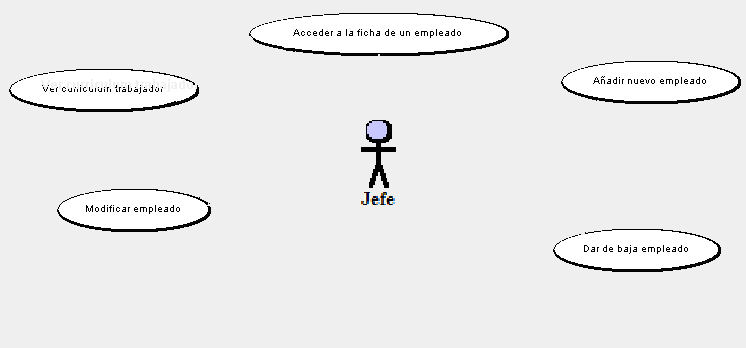
\includegraphics{Empleados}}
		
			\begin{itemize}
			\item \textbf{Actores: } Jefe.
			\item \textbf{Descripción: } La gestión de los empleados será realizada por el jefe. Éste poseerá una base de datos que englobará a todos ellos. Para cada empleado se tendrán los siguientes campos:
				\begin{itemize}
				\item 	 Nombre y apellidos
				\item 	 DNI
				\item 	 Puesto o labor que desempeña
				\item 	 Horario
				\item 	 Salario
				\item 	 Vacaciones
				\item 	 Fecha de entrada al negocio
				\item 	 Historial
				\item 	 Comentarios
				\end {itemize}
			\item \textbf{Incluye ($<<$include$>>$):} Añadir empleado, dar de baja a un empleado, modificar la ficha de un empleado.
		\end {itemize}
El único que tendrá acceso a esa base de datos (y por tanto el encargado de modificarla) será el jefe. Los antiguos empleados (que ya no trabajen en el negocio) también se encontrarán en la base de datos, en su correspondiente sección.
		
%ACCEDER A LA FICHA DE UN EMPLEADO

	\subsection{Acceder a la ficha de un empleado}		
			\begin{itemize}
			\item \textbf{Actor:} Jefe, empleados.
			\item \textbf{Propósito: } Acceder a la ficha de un determinado empleado.
			\item \textbf{Visión general:} El jefe accede al programa de gestión de empleados desde su ordenador. Después de introducir su nombre de usuario y su contraseña, accede a la base de datos de los empleados. En el buscador introduce el nombre deseado. Consulta su ficha y cierra la aplicación. \\
Para cada empleado se tendrán los siguientes campos:
				\begin{itemize}
				\item 	 Nombre y apellidos
				\item 	 DNI
				\item 	 Puesto o labor que desempeña
				\item 	 Horario
				\item 	 Salario
				\item 	 Vacaciones
				\item 	 Fecha de entrada al negocio
				\item 	 Historial
				\item 	 Comentarios
				\end {itemize}
			\item \textbf{Curso típico de eventos:} 	\\
				\begin{tabular}{|p{6cm}||p{6cm}|}
				\hline
				\textbf{Acción del actor} & \textbf{Respuesta del sistema} \\ \hline \hline
				\textbf{1.} El Log in ha sido realizado satisfactoriamente & \textbf{2.}Presenta las pestañas disponibles.\\ \hline 
				\textbf{3.} Selecciona la pestaña “Empleados”. & \textbf{4.} Muestra la pestaña, con las opciones correspondientes. \\ \hline
				\textbf{5.} Busca el nombre del empleado.	& \textbf{6.} Procesa la búsqueda y muestra la ficha del empleado. \\ \hline
				\textbf{7.} Se desplaza al apartado correspondiente.  & \textbf{} \\ \hline
				 \textbf{8.} Consulta el horario.  & \textbf{}\\ \hline
				\textbf{9.} Cierra la aplicación. & \textbf{} \\ \hline
			\end{tabular}
			\\
			\item \textbf{Cursos alternativos:} 
			\begin{itemize}
			\item  \textbf{Línea 8:} No existe un empleado actual con ese nombre. Se ofrecen al administrador 2 opciones: Introducir otro nombre o buscar por NIF.
			\end {itemize}
		\end{itemize}%FIn de caso de uso


%AÑADIR CLIENTE
	\newpage
	\subsection{Añadir cliente}
		
		\hspace{-1.2 true cm}	
			\scalebox{0.7}{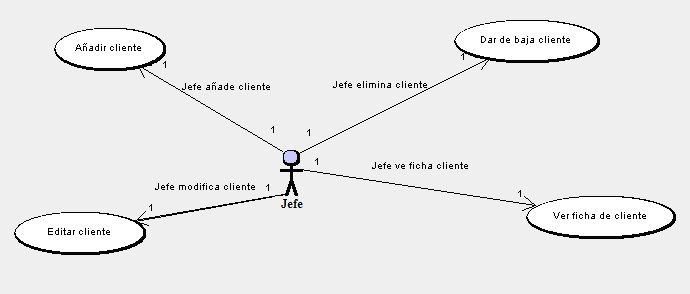
\includegraphics{Cliente}} 
			\begin{itemize}
			\item \textbf{Actor:} Jefe, recepcionista, maître.
			\item \textbf{Propósito: } Crear una nueva ficha de cliente.
			\item \textbf{Visión general:} El actor accede al programa de gestión de empleados desde su equipo, y entra en la base de datos de los clientes. Rellena la ficha con los datos del cliente. Tras haberla completado, comprueba que los datos introducidos son correctos. Cierra la aplicación. 
			\item \textbf{Curso típico de eventos:} 	\\
				\begin{tabular}{|p{6cm}||p{6cm}|}
				\hline
				\textbf{Acción del actor} & \textbf{Respuesta del sistema} \\ \hline \hline
				\textbf{1.} El Log in ha sido realizado satisfactoriamente & \textbf{2.}Presenta las pestañas disponibles.\\ \hline 
				\textbf{3.} Selecciona la pestaña “Clientes”. & \textbf{4.} Muestra la pestaña, con las opciones correspondientes. \\ \hline
				\textbf{5.} Clica en ''Añadir cliente".	& \textbf{6.} Muesta la ficha a rellenar. \\ \hline
				\textbf{7.} Rellena la ficha. & \textbf{8.} Se asegura de que todos los campos obligatorios están completos y muestra los datos del nuevo cliente para comprobar que son correctos.\\ \hline
				\textbf{9.} Lo comprueba y cierra la aplicación. & \textbf{} \\ \hline
			\end{tabular}
			\\
			\item \textbf{Cursos alternativos:} 
			\begin{itemize}
			\item  \textbf{Línea 8:} Algún campo es incorrecto o está sin rellenar. El programa regresa a la línea 7.
			\item  \textbf{Línea 9:} El actor se ha equivocado al rellenar un campo. El programa le devuelve a la línea 7.
			\end {itemize}
		\end{itemize}%FIn de caso de uso


%VER FICHA DE CLIENTE

	\subsection{Ver ficha de cliente}
			\begin{itemize}
			\item \textbf{Actor:} Jefe, recepcionista, maître.
			\item \textbf{Propósito: } Acceder a la ficha de un cliente.
			\item \textbf{Visión general:} El actor entra al programa de gestión de empleados desde su ordenador, y accede a la base de datos de los clientes. Busca al cliente por nombre y/o apellidos . Una vez que lo encuentra, consulta los datos que desee. Cierra la aplicación. 
			\item \textbf{Curso típico de eventos:} 	\\
				\begin{tabular}{|p{6cm}||p{6cm}|}
				\hline
				\textbf{Acción del actor} & \textbf{Respuesta del sistema} \\ \hline \hline
				\textbf{1.} El Log in ha sido realizado satisfactoriamente. & \textbf{2.} Presenta las pestañas disponibles.\\ \hline
				\textbf{3.} Selecciona la pestaña “Clientes”. & \textbf{4.} Muestra la pestaña, con las opciones correspondientes. \\ \hline
				\textbf{5.} Clica en "Buscar cliente".	& \textbf{6.} Procesa la búsqueda y muestra la ficha del cliente. \\ \hline
				\textbf{7.} Consulta la ficha del cliente y cierra la aplicacion.& \\ \hline
				
			\end{tabular}
			\\
			\item \textbf{Cursos alternativos:} 
			\begin{itemize}
			\item  \textbf{Línea 6:} Ese cliente no existe, vuelve a la línea 5.
			\item  \textbf{Línea 5:} Tras pasar por el curso alternativo anterior y ver que el cliente no existe, sale de la aplicación.
			\end {itemize}
		\end{itemize}%FIn de caso de uso


%%%%LIMPIEZA (CASOS DE USO)

%ORGANIZAR TAREAS DE LIMPIEZA		
	\hspace{0.6 true cm}
	\scalebox{0.7}{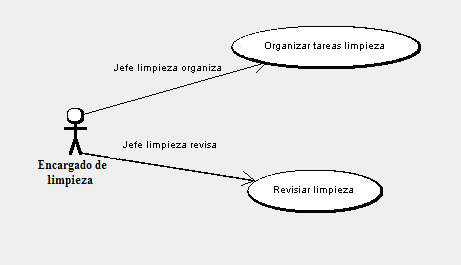
\includegraphics{OrganizacionLimpieza}}
	\subsection{Organizar tareas de limpieza}
			\begin{itemize}
			\item \textbf{Actor: }Jefe de limpieza.
			\item \textbf{Propósito: }Organizar las tareas de limpieza, repartiendo el trabajo entre los empleados de limpieza y organizando los horarios. 		
			\item \textbf{Visión general: }El jefe de limpieza accede al programa a través de su dispositivo. Debe introducir su nombre de usuario y contraseña. Una vez ha accedido, tiene la opción de organizar las tareas de limpieza. Pulsando esta opción puede crear una lista de tareas de limpieza, y repartir dichas tareas entre los trabajadores de limpieza. 
			\item \textbf{Curso típico de eventos:} \\	%El curso tipico de eventos se hace en dos columnas (Accion del actor 		Respuesta del sistema), es que no me acuerdo como se ponia el Latex las columnas, si eso recuadrado
\begin{tabular}{|p{6cm}||p{6cm}|}
				\hline
				\textbf{Acción del actor} & \textbf{Respuesta del sistema} \\ \hline \hline
				\textbf{1.} El Log in ha sido realizado satisfactoriamente. & \textbf{2.} Presenta las opciones disponibles.\\ \hline
				\textbf{3.} Selecciona la opción “Determinar lugares a limpiar”. & \textbf{4.} Muestra la pestaña, con las opciones correspondientes. \\ \hline
				\textbf{5.} Selecciona la opción de ''Crear tarea".	& \textbf{6.} Muestra los campos ''Lugar", ''Empleado'' y ''Comentarios". \\ \hline
				\textbf{7.}Rellena los campos . & \textbf{8.} Envía una notificación al personal de limpieza correspondiente con los campos que ha rellenado el encargado de limpieza.\\ \hline
				\textbf{9.}Cierra la aplicación. & \textbf{} \\ \hline
			\end{tabular}

			\item \textbf{Cursos alternativos:} 
				\begin {itemize}
					
					\item \textbf{Línea 8: } Al rellenar el campo del empleado, se elige uno que ha alcanzado el máximo de tareas a realizar en ese día. El sistema informa de esto, y el jefe debe volver a elegir a otro empleado.
				\end {itemize}
			\end{itemize}%Fin de caso de uso


%REVISAR LIMPIEZA

\subsection{Revisar limpieza}
			\begin{itemize}
			\item \textbf{Actor: }Jefe de limpieza.
			\item \textbf{Propósito: }Da la posibilidad al encargado de limpieza de comprobar que aquellos lugares que ya han sido marcados como "limpiados" por los trabajadores de limpieza, efectivamente lo están.  		
			\item \textbf{Visión general: }Anteriormente, el jefe ha creado una lista de tareas, que pueden consultar los trabajadores de limpieza. Cada vez que se limpia un sitio, este se tacha de la lista de "Sitios por limpiar" y se añade a la de "Sitios limpiados".  
			\item \textbf{Curso típico de eventos:}\\ 	%El curso tipico de eventos se hace en dos columnas (Accion del actor 		Respuesta del sistema), es que no me acuerdo como se ponia el Latex las columnas, si eso recuadrado
\begin{tabular}{|p{6cm}||p{6cm}|}
				\hline
				\textbf{Acción del actor} & \textbf{Respuesta del sistema} \\ \hline \hline
				\textbf{1.} El Log in ha sido realizado satisfactoriamente. & \textbf{2.} Presenta las pestañas disponibles.\\ \hline
				\textbf{3.} Selecciona la pestaña “Revisión de limpieza”. & \textbf{4.} Muestra la lista de los sitios que han sido limpiados. \\ \hline
				\textbf{5.} Va marcando en la lista aquellos sitios que ha comprobado que están limpios.	& \textbf{6.} Elimina de la lista los sitios marcados. \\ \hline
				\textbf{7.} En aquellos sitios que no están limpios del todo, o en los que falta algo, puede pulsar la opción de ''Agregar comentario". & \textbf{8.} Envía el comentario al personal de limpieza. El sitio se vuelve a añadir a la lista de "Sitios por limpiar".\\ \hline
				\textbf{9.}Cierra la aplicación. & \textbf{} \\ \hline
			\end{tabular}
			\item \textbf{Cursos alternativos:} 
				\begin{itemize}
					\item \textbf{Línea 9: }Si el comentario excede los 140 caracteres, el sistema informará de ésto al usuario, que podrá editar su comentario para que no exceda los 140 caracteres.
				\end{itemize}
		\end {itemize}

%CONSULTAR TAREAS

	\hspace{0.7 true cm}
	\scalebox{0.9}{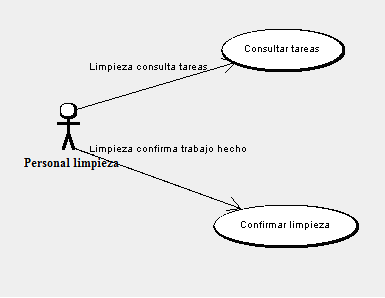
\includegraphics{Limpieza}} 
	\subsection{Consultar tareas}				
			\begin{itemize}
				\item \textbf{Actor: } Personal de limpieza.
				\item \textbf{Visión general: } Permite al personal de limpieza consultar las tareas que el encargado de limpieza les ha asignado. 		
			\end {itemize}

%CONFIRMAR LIMPIEZA DE HABITACION

	
		\subsection{Confirmar limpieza de habitación}
			\begin{itemize}
			\item \textbf{Actor: } Personal de limpieza.
			\item \textbf{Propósito: }Eliminar de la lista de tareas una tarea que ha sido completada.
			\item \textbf{Visión general: }El jefe de limpieza envía a los trabajadores de limpieza una lista con las tareas que deben hacer. Una vez que estas tareas han sido realizadas, los trabajadores de limpieza deben eliminarlas de la lista de "Tareas por realizar".
			\item \textbf{Curso típico de eventos:}\\ 	%El curso tipico de eventos se hace en dos columnas (Accion del actor 		Respuesta del sistema), es que no me acuerdo como se ponia el Latex las columnas, si eso recuadrado
				\begin{tabular}{|p{6cm}||p{6cm}|}
					\hline
					\textbf{Acción del actor} & \textbf{Respuesta del sistema} \\ \hline \hline
					\textbf{1.} Selecciona el botón  ''Confirmar limpieza de habitación". & \textbf{2.}Muestra la lista de tareas que el usuario debía realizar.\\ \hline 
					\textbf{3.}El usuario selecciona aquellas tareas que ha completado. & \textbf{4.} Presenta el botón de ''Aceptar".\\ \hline
					\textbf{5.} Pulsa el botón de aceptar. & \textbf{6.} Las tareas elegidas se eliminan de la lista de "Tareas a realizar". \\ \hline
					\textbf{7.} Cierra la aplicación.	& \\ \hline	
				\end{tabular}
			\item \textbf{Cursos alternativos:} 
				\begin{itemize}
					\item \textbf{Línea 3: } Puede que el trabajador no haya podido realizar una tarea en el momento en el que le fue propuesta (por ejemplo, habitación con "no molestar").
 En este caso, puede elegir una opción que diga ''Recordar para más tarde".
				\end{itemize}
		\end {itemize}%FIn de caso de uso

%INFORMAR DE INCIDENCIAS

		\subsection{Anotar incidencias}	
			\begin{itemize}
				\item \textbf{Actor: } Todos los usuarios.
				\item \textbf{Propósito: } Informar de incidencias de mantenimiento que requieran de reparación. 		
				\item \textbf{Visión general: } Cuando se detecta una avería, o alguna otra incidencia de mantenimiento, se informa de ésta al encargado de mantenimiento a través de la aplicación.  
				\item \textbf{Curso típico de eventos:}\\ 
				\begin{tabular}{|p{6cm}||p{6cm}|}
					\hline
					\textbf{Acción del actor} & \textbf{Respuesta del sistema} \\ \hline \hline
					\textbf{1.} Selecciona el botón "Notificar incidencia" & \textbf{2.}Muestra los campos "Lugar'' y "Descripción".\\ \hline 
					\textbf{3.} Rellena dichos campos y pulsa el tick para aceptar. & \textbf{4.} Envía la notificación al encargado de mantenimiento.\\ \hline
					\textbf{5.} Cierra sesión. & \\ \hline

				\end{tabular}
				\item \textbf{Cursos alternativos:} 
					\begin{itemize}
						\item \textbf{Línea 3: }El usuario tiene la opción de ''Cancelar". Si pulsa esta opción la notificación no se enviará y el usuario volverá a su pantalla principal.
					\end{itemize}
			\end {itemize}

%CONSULTAR TAREAS DE MANTENIMIENTO
		\hspace{-1.5 true cm}
		\scalebox{0.9}{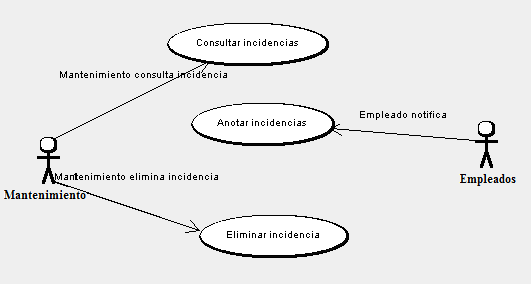
\includegraphics{Mantenimiento}} 
		\subsection{Consultar incidencias (manteniminento)}
			\begin{itemize}
			\item \textbf{Actor: }Encargado de mantenimiento.
			\item \textbf{Propósito: }Consultar incidencias de mantenimiento, y tachar de la lista aquellas incidencias que han sido resueltas. 
			\item \textbf{Visión general: }El personal del hotel informa al encargado de mantenimiento de incidencias que hayan ocurrido en el hotel a través de notificaciones. Cuando se resuelve una incidencia, el encargado de mantenimiento la elimina de su lista. 
			\item \textbf{Curso típico de eventos:}\\ 	%El curso tipico de eventos se hace en dos columnas (Accion del actor 		Respuesta del sistema), es que no me acuerdo como se ponia el Latex las columnas, si eso recuadrado
			\begin{tabular}{|p{6cm}||p{6cm}|}
				\hline
				\textbf{Acción del actor} & \textbf{Respuesta del sistema} \\ \hline \hline
				\textbf{1.} Selecciona el botón "Notificaciones". & \textbf{2.}Muestra la lista de incidencias que el resto de usuarios ha enviado.\\ \hline 
				\textbf{3.}El usuario selecciona aquellas tareas que ha completado. & \textbf{4.} Las tareas elegidas se eliminan de la lista de "Notificaciones pendientes".\\ \hline
				\textbf{5.} Cierra sesión. & \\ \hline
			\end{tabular}
		\end {itemize}
		
	% CASOS DE USO DE RESTAURANTE 
		
%RESERVAR MESA
		\newpage
		\hspace{-2.4 true cm}	
		\scalebox{0.65}{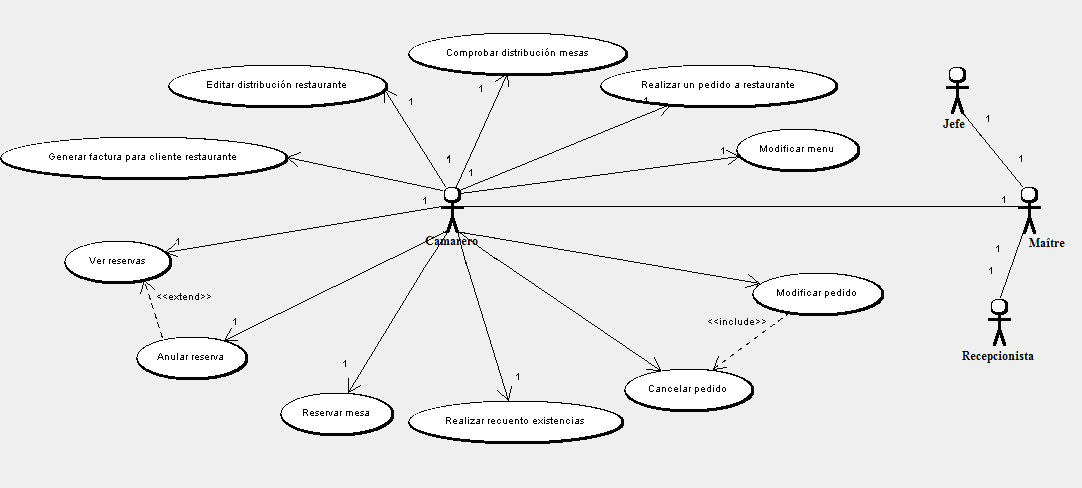
\includegraphics{Restaurante}}
		\subsection{Reservar mesa} 
			\begin{itemize}
			\item \textbf{Actor:} Camareros, maître, recepcionista, chef, cocineros.
			\item \textbf{Propósito: } Reservar una mesa en el restaurante para comer.
			\item \textbf{Visión general:} El empleado que va a realizar la reserva selecciona una de las mesas disponibles en función del número de comensales.
			\item \textbf{Curso típico de eventos:} 	\\
				\begin{tabular}{|p{6cm}||p{6cm}|}
				\hline
				\textbf{Acción del actor} & \textbf{Respuesta del sistema} \\ \hline \hline
				\textbf{1.}  El Log in ha sido realizado satisfactoriamente. & \textbf{2.} El programa da la bienvenida y le muestra las opciones. \\ \hline
				\textbf{3.} Selecciona la opción reservar mesa. & \textbf{4.} El programa pide que se introduzca el número de comensales. \\ \hline
				\textbf{5.} El usuario introduce el numero.	& \textbf{6.} Pide al usuario introducir una hora de llegada. \\ \hline
				\textbf{7.} El usuario introduce la hora de la reserva.	& \textbf{8.} Muestra la distribución de las mesas y marca de verde las disponibles. \\ \hline
				\textbf{9.} El usuario selecciona una mesa. & \textbf{10.} La aplicación muestra un mensaje indicando que la reserva se realizó correctamente. \\ \hline
				\textbf{11.} Cierra la aplicación. & \textbf{} \\ \hline
			\end{tabular}
			\\
			\item \textbf{Cursos alternativos:} 
			\begin{itemize}
			\item  \textbf{Línea 6:} El numero introducido es incorrecto. Se pide al usuario que introduzca otro numero. Si el usuario no desea continuar la reserva puede salir de la aplicación.
			\item  \textbf{Línea 8:} La hora introducida es incorrecta. Se pide al usuario que introduzca otra hora. Si el usuario no desea continuar la reserva puede salir de la aplicación.
			\item  \textbf{Línea 10:} El usuario selecciona una mesa no disponible. El Sistema indica que la mesa no esta disponible, y pide al usuario reservar otra mesa. Puede salir de la aplicación si no desea continuar la reserva.
			\end {itemize}
		\end {itemize}
		
%ANULAR RESERVA

		\subsection{Anular reserva}
			\begin{itemize}
			\item \textbf{Actor:} Camareros, maître, recepcionista, chef, cocineros.
			\item \textbf{Propósito: } Anular una reserva realizada con anterioridad.
			\item \textbf{Visión general:} El empleado que desea anular una reserva inicia la aplicación, se identifica y selecciona la reserva que se va a anular.
			\item \textbf{Extiende ($<<$extends$>>$):} Reservar Mesa
			\item \textbf{Curso típico de eventos:} 	\\
				\begin{tabular}{|p{6cm}||p{6cm}|}
				\hline
				\textbf{Acción del actor} & \textbf{Respuesta del sistema} \\ \hline \hline
				\textbf{1.}  El Log in ha sido realizado satisfactoriamente. & \textbf{2.} El programa da la bienvenida y le muestra las opciones. \\ \hline
				\textbf{3.} Selecciona la opción anular reserva, dentro de la pestaña ''Restaurante". & \textbf{4.} El programa muestra las mesas reservadas, incluyendo hora y numero de comensales. \\ \hline
				\textbf{5.} El usuario selecciona la reserva que desea anular	& \textbf{6.} Se muestra un mensaje con los datos completos de la reserva (hora, comensales, propietario de la reserva...) para verificar que realmente se desea anular. \\ \hline
				\textbf{7.} Selecciona continuar.	& \textbf{8.} La aplicación muestra un mensaje indicando que la anulación se realizó correctamente. \\ \hline
				\textbf{9.} Cierra la aplicación. & \textbf{} \\ \hline
			\end{tabular}
			\\
			\item \textbf{Cursos alternativos:} 
			\begin{itemize}
			\item  \textbf{Línea 7:} El usuario selecciona Cancelar. La reserva no se anula. Puede elegir entre anular otra reserva o salir.
			\end {itemize}
		\end {itemize}
	
%GENERAR UN PEDIDO PARA UNA MESA

		\subsection{Generar un pedido para una mesa}
			\begin{itemize}
			\item \textbf{Actor:} Camareros, maître.
			\item \textbf{Propósito: } Pedir un plato a la cocina.
			\item \textbf{Visión general:} El camarero o el maître realiza la petición de un plato directamente a la cocina.
			\item \textbf{Curso típico de eventos:} 	\\
				\begin{tabular}{|p{6cm}||p{6cm}|}
				\hline
				\textbf{Acción del actor} & \textbf{Respuesta del sistema} \\ \hline \hline
				\textbf{1.} El empleado reactiva la aplicación (normalmente queda en pausa porque no va a encenderlo cada vez que pide un plato). & \textbf{2.} Muestra las opciones.\\ \hline 
				\textbf{3.} Introduce la opcion generar un pedido. & \textbf{4.} Pide que introduzca los platos deseados. \\ \hline
				\textbf{5.} Puede introducir un plato de la carta y personalizarlo introduciendo o eliminando ingredientes. & \textbf{6.} Da la opción al usuario de introducir más platos o terminar. \\ \hline
				\textbf{7.} Selecciona no realizar más pedidos.	& \textbf{8.} El programa manda el pedido a la cocina. \\ \hline
				\textbf{9.} El empleado pone la aplicación en pausa. & \\ \hline
			\end{tabular}
			\\
			\item \textbf{Cursos alternativos:} 
			\begin{itemize}
			\item  \textbf{Línea 5:} El plato introducido no existe. Se muestra un mensaje de error y se da la opción de seguir o terminar el pedido.
			\item  \textbf{Línea 5:} Se ha introducido un plato de forma incorrecta y el camarero lo elimina o lo modifica.
			\end {itemize}
		\end {itemize}
		
%MODIFICAR UN PEDIDO
		
	\subsection{Modificar un pedido}
			\begin{itemize}
			\item \textbf{Actores:} Camareros, maître.
			\item \textbf{Descripción:} Se pueden acceder a los pedidos realizados por un cliente y modificarlos, en caso de que no se trate de lo que ellos deseaban.
		\end {itemize}


%CANCELAR UN PEDIDO

		\subsection{Cancelar un pedido}
			\begin{itemize}
			\item \textbf{Actor:} Camareros, maître.
			\item \textbf{Propósito: } Anular un pedido realizado.
			\item \textbf{Visión general:} El cliente puede pedir a un empleado que anule un pedido que realizó siempre que no haya comenzado a prepararse.
			\item \textbf{Extiende ($<<$extends$>>$):} Generar un pedido.
			\item \textbf{Curso típico de eventos:} 	\\
				\begin{tabular}{|p{6cm}||p{6cm}|}
				\hline
				\textbf{Acción del actor} & \textbf{Respuesta del sistema} \\ \hline \hline
				\textbf{1.} El empleado hace Log in satisfactoriamente. & \textbf{2.} Muestras las opciones que puede realizar. \\ \hline
				\textbf{3.} Selecciona la opción cancelar pedido, dentro de la pestaña ''Restaurante". & \textbf{4.} Muestra todos los pedidos. \\ \hline
				\textbf{5.} Selecciona el pedido que desea anular	& \textbf{6.} Se muestra un mensaje con los datos del pedido para verificar que realmente se desea anular. \\ \hline
				\textbf{7.} Selecciona continuar.	& \textbf{8.} La aplicación muestra un mensaje indicando que la anulación se realizó correctamente. \\ \hline
				\textbf{9.} Cierra la aplicación. &  \\ \hline
			\end{tabular}
			\\
			\item \textbf{Cursos alternativos:} 
			\begin{itemize}
			\item  \textbf{Línea 7:} El usuario selecciona cancelar. La reserva no se anula. Puede elegir entre anular otra reserva o salir.
			\end {itemize}
		\end {itemize}
		
%GENERAR FACTURA A UN CLIENTE

		\subsection{Generar factura a un cliente}
			\begin{itemize}
			\item \textbf{Actor:} Camareros, maître.
			\item \textbf{Propósito: } Proporcionar la factura para cobrar al cliente.
			\item \textbf{Visión general:} Se selecciona el cliente del cual se desea obtener la factura y se imprime. Se da la opción al cliente de pagar en el momento o que se lo carguen en la cuenta de la habitación, si es que está alojado en el hotel.
			\item \textbf{Curso típico de eventos:} 	\\
				\begin{tabular}{|p{6cm}||p{6cm}|}
				\hline
				\textbf{Acción del actor} & \textbf{Respuesta del sistema} \\ \hline \hline
				\textbf{1.}   El empleado hace Log in satisfactoriamente. & \textbf{2.} Muestras las opciones que puede realizar. \\ \hline
				\textbf{3.} Selecciona la opción generar factura, dentro de la pestaña ''Restaurante''. & \textbf{4.} Muestra las mesas ocupadas de las cuales aún no se ha obtenido la factura. \\ \hline
				\textbf{5.} Selecciona la mesa a cobrar.	& \textbf{6.} Se muestra un mensaje con el número de mesa, todos los pedidos realizados y el precio. \\ \hline
				\textbf{7.} Selecciona imprimir.	& \textbf{8.} La aplicación muestra un mensaje indicando que la factura se imprimió. \\ \hline
				\textbf{9.} El empleado cobre al cliente.	& \textbf{10.} Muestra un mensaje de ''Cobrado con éxito''. \\ \hline
				\textbf{11.} Cierra la aplicación. &  \\ \hline
			\end{tabular}
			\\
			\item \textbf{Cursos alternativos:} 
			\begin{itemize}
			\item  \textbf{Línea 7:} El usuario selecciona Cancelar. No se genera la factura.
			\item  \textbf{Línea 10:} El cobro no se ha realizado con éxito. La mesa sigue con deudas.
			\end {itemize}
		\end {itemize}
		
%VER MENU		
 	
	\subsection{Ver menú}
			\begin{itemize}
			\item \textbf{Actores:} Camareros, maître, cocineros, chef y jefe.
			\item \textbf{Descripción:} Muestra pon pantalla el menú ordenado por tipo de plato. En cada plato se puede pinchar para obtener una descripción del plato más precisa. Los platos se ordenarán del siguiente modo:
			\begin{itemize}
				\item 	 Entrantes
				\item 	 Principales
				\item 	 Segundos
				\item 	 Postres
				\end {itemize}
		\end {itemize}

%AÑADIR NOTA
	\newpage
	\hspace{0.5 true cm}	
	\scalebox{0.8}{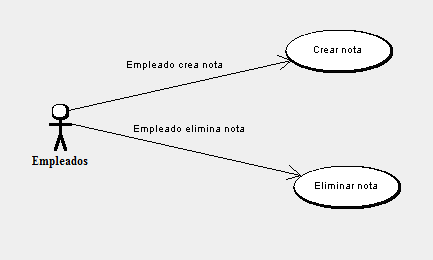
\includegraphics{Notas}}
	\subsection{Añadir nota} 
			\begin{itemize}
			\item \textbf{Actor:} Todos.
			\item \textbf{Propósito: } Crear una nota y añadirla al tablón.
			\item \textbf{Visión general:} Las notas son el principal medio de comunicación escrito entre los empleados del negocio. 		Así pues, todos tendrán acceso a esta pestaña y podrán subir sus notas y ver las de los demás. La
pestaña de notas es la única común a todos los empleados.
			\item \textbf{Curso típico de eventos:} 	\\
				\begin{tabular}{|p{6cm}||p{6cm}|}
				\hline
				\textbf{Acción del actor} & \textbf{Respuesta del sistema} \\ \hline \hline
				\textbf{1.}    El empleado hace Log in satisfactoriamente. & \textbf{2.} Muestras las opciones que puede realizar. \\ \hline
				\textbf{3.} Selecciona la opción notas. & \textbf{4.} Muestra el tablón de notas. \\ \hline
				\textbf{5.} Selecciona la opción ''Crear nota".	& \textbf{6.} Se muestra el cuadro de texto a rellenar. \\ \hline
				\textbf{7.} Escribe la nota.	& \textbf{8.}Muestra el tablón de notas con la nueva nota añadida. \\ \hline
				\textbf{9.} Cierra la aplicación. &  \\ \hline
			\end{tabular}
			\\
			\item \textbf{Cursos alternativos:} No hay cursos alternativos para este caso de uso.
		\end {itemize}


%BORRAR NOTA
		\subsection{Borrar nota}
			\begin{itemize}
			\item \textbf{Actor:} Todos.
			\item \textbf{Propósito: } Borra una nota del tablón.
			\item \textbf{Visión general:} Selecciona una nota del tablón y la elimina, tanto para él como para el resto de empleados.
			\item \textbf{Curso típico de eventos:} 	\\
				\begin{tabular}{|p{6cm}||p{6cm}|}
				\hline
				\textbf{Acción del actor} & \textbf{Respuesta del sistema} \\ \hline \hline
				\textbf{1.}    El empleado hace Log in satisfactoriamente. & \textbf{2.} Muestras las opciones que puede realizar. \\ \hline
				\textbf{3.} Selecciona la opción notas. & \textbf{4.} Muestra el tablón de notas. \\ \hline
				\textbf{5.} Selecciona una nota y la elimina.	& \textbf{6.} La aplicación pregunta: "¿Está seguro que desea eliminar esta nota?. \\ \hline
				\textbf{7.} Confirma.	& \textbf{8.}Muestra el tablón de notas, sin la nota recién eliminada. \\ \hline
				\textbf{9.} Cierra la aplicación. &  \\ \hline
			\end{tabular}
			\\
			\item \textbf{Cursos alternativos:} 
			\begin{itemize}
			\item  \textbf{Línea 7:}El usuario no quiere eliminar la nota. la aplicación vuelve a la línea 6.
			\end {itemize}
		\end {itemize}

%VER CUENTA DIARIA DE LA CAJA DE RECEPCIÓN.
	
	\hspace{-2 true cm}
	\scalebox{0.6}{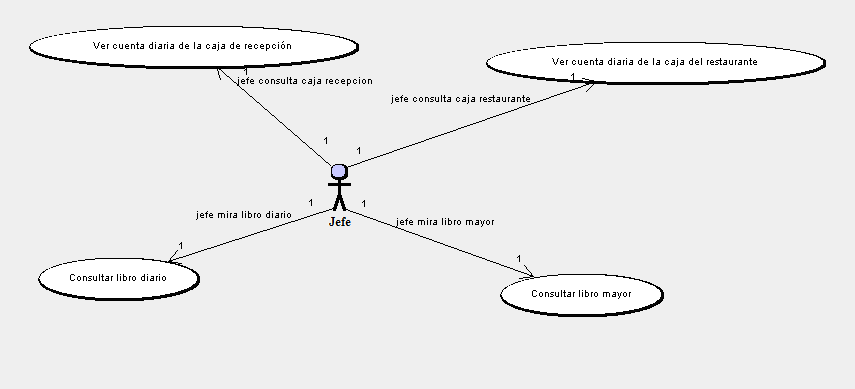
\includegraphics{Contabilidad}} 
	\subsection{Ver cuenta diaria de la caja de recepción}
		\begin{itemize}
			\item \textbf{Actor:} Jefe.
			\item \textbf{Descrición:} El jefe ve los flujos de caja que se han producido durante el día, y la cantidad que debe haber en la caja de la recepción.	
		\end {itemize}

%VER CUENTA DIARIA DE LA CAJA DEL RESTAURANTE.

	\subsection{Ver cuenta diaria de la caja del restaurante}
		\begin{itemize}
			\item \textbf{Actor:} Jefe.
			\item \textbf{Descrición:} El jefe ve los flujos de caja que se han producido durante el día, y la cantidad que debe haber en la caja del restaurante.	
		\end {itemize}

%CONSULTAR LIBRO DIARIO

	\subsection{Consultar libro diario}
		\begin{itemize}
			\item \textbf{Actor:} Jefe.
			\item \textbf{Descrición:} El jefe ve los últimos apuntes del libro diario, pudiendo ascender si lo desea hasta el asiento de apertura.	
		\end {itemize}

%CONSULTAR LIBRO MAYOR

	\subsection{Consultar libro mayor}
		\begin{itemize}
			\item \textbf{Actor:} Jefe.
			\item \textbf{Descrición:} El jefe ve los últimos apuntes en las cuentas del libro mayor. \\
		\end {itemize}

%VER HABITACIONES
	
	\hspace{-2 true cm}
	\scalebox{0.65}{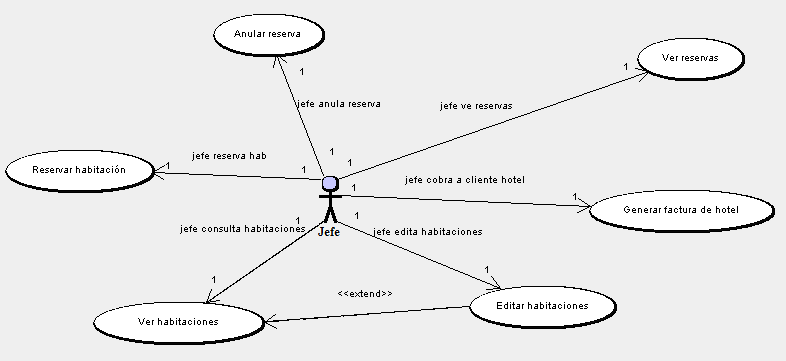
\includegraphics{Habitaciones}}
	\subsection{Ver habitaciones}
		\begin{itemize}
			\item \textbf{Actor:} Recepcionista, maître, jefe.
			\item \textbf{Propósito: } Ver las características de las habitaciones del hotel
			\item \textbf{Visión general:} Se muestran las características de cada habitación seleccionada.
			\item \textbf{Incluye ($<<$include$>>$):} Modificar habitaciones.
			\item \textbf{Curso típico de eventos:} 	\\
				\begin{tabular}{|p{6cm}||p{6cm}|}
				\hline
				\textbf{Acción del actor} & \textbf{Respuesta del sistema} \\ \hline
				\textbf{1.} Pincha en la pestaña de habitaciones & \textbf{2.}Se muestra la sección habitaciones.\\ \hline 
				\textbf{3.} Selecciona ver habitaciones. & \textbf{4.}Se muestran las características de la primera habitación  \\ \hline
				\textbf{5.} Se selecciona otra habitación & \textbf{6.} Se muestran las características de la habitación seleccionada. \\ \hline
				\textbf{7.} Continúa en la ventana hasta que se selecciona otra pestaña. & \\ \hline
			\end{tabular}
			\\
		\end {itemize}
		
%RESERVAR HABITACION
	\subsection{Reservar habitacion}
		\begin{itemize}
			\item \textbf{Actor:} Recepcionista, maître, jefe.
			\item \textbf{Propósito: } Reservar una habitación del hotel.
			\item \textbf{Visión general:} Cuando un cliente reserva una habitación, se guarda toda la información de la reserva.
			\item \textbf{Curso típico de eventos:} 	\\
				\begin{tabular}{|p{6cm}||p{6cm}|}
				\hline
				\textbf{Acción del actor} & \textbf{Respuesta del sistema} \\ \hline
				\textbf{1.} Pincha en la pestaña de habitaciones & \textbf{2.}Se muestra la sección habitaciones.\\ \hline 
				\textbf{3.} Selecciona realizar reserva. & \textbf{4.}Se muestran los campos a completar  \\ \hline
				\textbf{5.}Rellena los campos deseados & \textbf{6.} Se muestran las opciones elegidas y la disponibilidad de la habitación elegida \\ \hline
				\textbf{7.} Se confirma la reserva & \textbf{8.}Regresa a la pantalla general de habitaciones\\ \hline
			\end{tabular}
			\\
			\item \textbf{Cursos alternativos:} 
			\begin{itemize}
			\item  \textbf{Línea 5:} La habitación seleccionada no está libre, se deberá elegir otra.
			\item  \textbf{Línea 7:} Se cancela la reserva. \\
			\end {itemize}
		\end {itemize}

%VER RESERVAS
	\subsection{Ver reservas}
		\begin{itemize}
			\item \textbf{Actor:} Recepcionista, maître, jefe.
			\item \textbf{Propósito: } Ver la reserva de habitaciones del hotel.
			\item \textbf{Visión general:} Se ve el total de las futuras reservas de habitaciones del hotel ordenadas por fecha.
			\item \textbf{Incluye ($<<$include$>>$):} Anular reserva.
			\item \textbf{Curso típico de eventos:} 	\\
				\begin{tabular}{|p{6cm}||p{6cm}|}
				\hline
				\textbf{Acción del actor} & \textbf{Respuesta del sistema} \\ \hline
				\textbf{1.} Pincha en la pestaña de habitaciones & \textbf{2.}Se muestra la sección habitaciones \\ \hline 
				\textbf{3.} Selecciona ver/anular reservas. & \textbf{4.}Se muestran la lista de reservas \\ \hline
			\end{tabular}
			\\
		\end {itemize}

%ANULAR RESERVAS

	\subsection{Anular reservas}
		\begin{itemize}
			\item \textbf{Actor:} Recepcionista, maître, jefe.
			\item \textbf{Descrición:}Desde la pantalla de ver reservas, se permite anular la reserva deseada. 		
		\end {itemize}

%GENERAR FACTURA DEL HOTEL

	\subsection{Generar factura del hotel}
		\begin{itemize}
			\item \textbf{Actor:} Recepcionista, maître, jefe.
			\item \textbf{Propósito: } Generar una factura para un cliente.
			\item \textbf{Visión general:}Cuando un cliente quiere pagar la factura del hotel, se genera la factura correspondiente.
			\item \textbf{Curso típico de eventos:} 	\\
				\begin{tabular}{|p{6cm}||p{6cm}|}
				\hline
				\textbf{Acción del actor} & \textbf{Respuesta del sistema} \\ \hline
				\textbf{1.} Pincha en la pestaña de habitaciones & \textbf{2.}Se muestra la sección habitaciones \\ \hline 
				\textbf{3.} Selecciona generar factura & \textbf{4.}Se muestran los campos de la factura.  \\ \hline
				\textbf{5.} Se modifican los campos deseados & \textbf{6.} Se muestra la factura final \\ \hline
				\textbf{7.} Se confirma generar factura & \textbf{8.}Regresa a la pantalla general de habitaciones\\ \hline
			\end{tabular}
			\\
		\end {itemize}

\newpage
%%%%%%CASOS DE USO SECUNDARIOS%%%%%%_____________________________________________________________________________________________________________________________________________________

\section{Secundarios}	

%AÑADIR EMPLEADO

	\subsection{Añadir un nuevo empleado}	
			\begin{itemize}
			\item \textbf{Actor:} Jefe.
			\item \textbf{Propósito: } Crear una nueva ficha de empleado.
			\item \textbf{Visión general:} El jefe accede a la aplicacion desde su ordenador. Después de introducir su nombre de usuario y su contraseña, accede a la base de datos de los empleados. Rellena la ficha con los datos del nuevo trabajador. Tras haberla completado, comprueba que los datos introducidos son correctos. Cierra la aplicación. 
			\item \textbf{Curso típico de eventos:} 	\\
				\begin{tabular}{|p{6cm}||p{6cm}|}
				\hline
				\textbf{Acción del actor} & \textbf{Respuesta del sistema} \\ \hline \hline
				\textbf{1.}   El empleado hace Log in satisfactoriamente. & \textbf{2.} Presenta las pestañas disponibles.\\ \hline
				\textbf{3.} Selecciona la pestaña “Empleados actuales”. & \textbf{4.} Muestra la pestaña, con las opciones correspondientes. \\ \hline
				\textbf{5.} Clica en ''Añadir empleado".	& \textbf{6.} Muesta la ficha a rellenar. \\ \hline
				\textbf{7.}Rellena la ficha. & \textbf{8.} Se asegura de que todos los campos obligatorios están completos y muestra los datos del nuevo cliente para comprobar que son correctos.\\ \hline
				\textbf{9.}Lo comprueba y cierra la aplicación. & \textbf{} \\ \hline
			\end{tabular}
			\\
			\item \textbf{Cursos alternativos:} 
			\begin{itemize}
			\item  \textbf{Línea 6:}Algún campo es incorrecto o está sin rellenar. El programa regresa a la línea 7.
			\item  \textbf{Línea 7:}El jefe se ha equivocado al rellenar un campo. El programa le devuelve a la línea 7.
			\end {itemize}
		\end{itemize}%FIn de caso de uso





%DAR DE BAJA A UN EMPLEADO

	\subsection{Dar de baja a un empleado}	
			\begin{itemize}
			\item \textbf{Actor:} Jefe, empleado.
			\item \textbf{Propósito: } Transferir la ficha de un empleado de "Empleados actuales" a "Antiguos empleados" .
			\item \textbf{Visión general:} El jefe accede a la aplicación desde su ordenador. Después de introducir su nombre de usuario y su contraseña, accede a la base de datos de los empleados. Busca un empleado y da de baja su ficha. Cierra la aplicación. 
			\item \textbf{Curso típico de eventos:} 	\\
				\begin{tabular}{|p{6cm}||p{6cm}|}
				\hline
				\textbf{Acción del actor} & \textbf{Respuesta del sistema} \\ \hline \hline
				\textbf{1.}   El empleado hace Log in satisfactoriamente. & \textbf{2.} Presenta las pestañas disponibles.\\ \hline
				\textbf{3.} Selecciona la pestaña “Empleados”. & \textbf{4.} Muestra la pestaña, con las opciones correspondientes. \\ \hline
				\textbf{5.} Clica en "Buscar empleado".	& \textbf{6.} Procesa la búsqueda y muestra la ficha del empleado. \\ \hline
				\textbf{7.}Selecciona "Dar de baja a este empleado". & \textbf{8.}Pide confirmación para dar de baja al empleado.\\ \hline
				\textbf{9.}Confirma. & \textbf{} \\ \hline
				\textbf{10.}Cierra la aplicación. & \textbf{} \\ \hline
			\end{tabular}
			\\
			\item \textbf{Cursos alternativos:} 
			\begin{itemize}
			\item  \textbf{Línea 6:}El empleado buscado no se encuentra en la base de datos. El programa le devuelve a la línea 5.
			\end {itemize}
		\end{itemize}%FIn de caso de uso


%MODIFICAR LA FICHA DE UN EMPLEADO

	\subsection{Modificar la ficha de un empleado}		
			\begin{itemize}
			\item \textbf{Actor:} Jefe.
			\item \textbf{Propósito: } Acceder a la ficha de un empleado y modificarla" .
			\item \textbf{Visión general:} El jefe accede a la aplicación desde su ordenador. Después de introducir su nombre de usuario y su contraseña, accede a la base de datos de los empleados. Busca un empleado, accede a su ficha y la modifica. Cierra la aplicación. 
	\newpage
			\item \textbf{Curso típico de eventos:} 	\\
				\begin{tabular}{|p{6cm}||p{6cm}|}
				\hline
				\textbf{Acción del actor} & \textbf{Respuesta del sistema} \\ \hline \hline
				\textbf{1.}   El empleado hace Log in satisfactoriamente. & \textbf{2.} Presenta las pestañas disponibles.\\ \hline
				\textbf{3.} Selecciona la pestaña “Empleados”. & \textbf{4.} Muestra la pestaña, con las opciones correspondientes. \\ \hline
				\textbf{5.} Clica en "Buscar empleado".	& \textbf{6.} Procesa la búsqueda y muestra la ficha del empleado. \\ \hline
				\textbf{7.}Selecciona "Modificar ficha". & \textbf{8.}Muestra la ficha lista para su modificacion.\\ \hline
				\textbf{9.}Cambia los campos que considere. & \textbf{10.} Muestra la ficha con los cambios realizados \\ \hline
				\textbf{11.}Comprueba que los cambios son correctos y cierra la aplicación. & \textbf{} \\ \hline
			\end{tabular}
			\\
			\item \textbf{Cursos alternativos:} 
			\begin{itemize}
			\item  \textbf{Línea 6:} El empleado buscado no se encuentra en la base de datos. El programa le devuelve a la línea 7.
			\item  \textbf{Línea 10:} Algún cambio realizado no es correcto. El programa le devuelve a la línea 9.
			\item  \textbf{Línea 11:}El jefe se ha equivocado al introducir algún dato y desea volver a modificar la ficha. El programa le devuelve a la línea 5.
			
			\end {itemize}
		\end{itemize}%FIn de caso de uso


%VER CURRICULUM DE EMPLEADO

	\subsection{Ver el currículum de un empleado}		
			\begin{itemize}
			\item \textbf{Actor:} Jefe.
			\item \textbf{Propósito: } Acceder al currículum vitae de un trabajador  .
			\item \textbf{Visión general:} El jefe accede a la aplicación desde su ordenador. Después de introducir su nombre de usuario y su contraseña, accede a la base de datos de los empleados. Busca un empleado, accede a su ficha y desde ahí a su currículum. Cierra la aplicación. 
			\item \textbf{Extiende ($<<$extends$>>$):} Log In, Ver ficha de empleado.
	\newpage
			\item \textbf{Curso típico de eventos:} 	\\
				\begin{tabular}{|p{6cm}||p{6cm}|}
				\hline
				\textbf{Acción del actor} & \textbf{Respuesta del sistema} \\ \hline \hline
				\textbf{1.}El jefe ha accedido correctamente a la ficha de un empleado. & \textbf{2.} Muestra los datos del empleado.\\ \hline
				\textbf{3.} Clica en "Ver curriculum".	& \textbf{4.} Muestra el curriculum del empleado. \\ \hline
				\textbf{5.}Lo consulta y cierra la aplicación. & \textbf{} \\ \hline
			\end{tabular}
			\\
			\item \textbf{Cursos alternativos:} No hay cursos alternativos para este caso de uso.
		\end{itemize}%FIn de caso de uso



%EDITAR CLIENTE

	\subsection{Editar cliente}		
			\begin{itemize}
			\item \textbf{Actor:} Jefe, recepcionista.
			\item \textbf{Propósito: } Editar la ficha de un cliente.
			\item \textbf{Visión general:} El actor accede al programa de gestión de empleados desde su equipo. Busca al cliente por nombre y/o apellidos. Se muestra la ficha del cliente, dando la opción de editar los campos que sean necesarios. Comprueba que las ediciones son correctas. Cierra la aplicación. 
			\item \textbf{Curso típico de eventos:} 	\\
				\begin{tabular}{|p{6cm}||p{6cm}|}
				\hline
				\textbf{Acción del actor} & \textbf{Respuesta del sistema} \\ \hline \hline
				\textbf{1.} El Log in ha sido realizado satisfactoriamente & \textbf{2.} Presenta las pestañas disponibles.\\ \hline 
				\textbf{3.} Selecciona la pestaña “Clientes”. & \textbf{4.} Muestra la pestaña, con las opciones correspondientes. \\ \hline
				\textbf{5.} Clica en "Buscar cliente".	& \textbf{6.} Muesta la ficha del cliente. \\ \hline
				\textbf{7.} Edita los campos que desee. & \textbf{8.} Se asegura de que el formato de los nuevos datos es correcto y muestra la ficha actualizada del cliente.\\ \hline
				\textbf{9.} Comprueba que los datos editados son correctos y cierra la aplicación. & \textbf{} \\ \hline
			\end{tabular}
			\\
			\item \textbf{Cursos alternativos:} 
			\begin{itemize}
			\item  \textbf{Línea 6:} Ese cliente no existe, vuelve a la línea 5.
			\item  \textbf{Línea 8:} Algún campo de los editados es incorrecto. El programa regresa a la línea 7.
			\item  \textbf{Línea 9:} El actor se ha equivocado al rellenar un campo. El programa le devuelve a la línea 7.
			\end {itemize}
		\end{itemize}%FIn de caso de uso


%DAR DE BAJA CLIENTE
	\subsection{Dar de baja cliente} 
			\begin{itemize}
			\item \textbf{Actor:} Jefe, recepcionista.
			\item \textbf{Propósito: } Elimina de la base de datos de clientes la ficha de un cliente.
			\item \textbf{Visión general:} El actor accede al programa de gestión de empleados desde su equipo. Después de introducir su nombre de usuario y su contraseña, accede a la base de datos de los clientes.  Busca al cliente por nombre y/o apellidos. Clica en "Eliminar a este cliente". El programa pide confirmación al actor de que realmente desea eliminar al cliente de la base de datos. Cierra la aplicación. 
			\item \textbf{Curso típico de eventos:} 	\\
				\begin{tabular}{|p{6cm}||p{6cm}|}
				\hline
				\textbf{Acción del actor} & \textbf{Respuesta del sistema} \\ \hline \hline
				\textbf{1.} El Log in ha sido realizado satisfactoriamente & \textbf{2.}Presenta las pestañas disponibles.\\ \hline 
				\textbf{3.} Selecciona la pestaña “Clientes”. & \textbf{4.} Muestra la pestaña, con las opciones correspondientes. \\ \hline
				\textbf{5.} Clica en "Buscar cliente".	& \textbf{6.} Muesta la ficha del cliente. \\ \hline
				\textbf{7.} Clica en ''Eliminar cliente". & \textbf{8.} Pide confirmación al actor.\\ \hline
				\textbf{9.} Confirma y cierra la aplicación. & \textbf{} \\ \hline
			\end{tabular}
			\\
			\item \textbf{Cursos alternativos:} 
			\begin{itemize}
			\item  \textbf{Línea 6:} Ese cliente no existe, vuelve a la línea 5.
			\item  \textbf{Línea 8:} El actor se ha equivocado y no desea eliminar al cliente de la base de datos. El programa le devuelve a la línea 6.
			\item  \textbf{Línea 9:} El actor se ha equivocado al rellenar un campo. El programa le devuelve a la línea 7.
			\end {itemize}
		\end{itemize}


%COMPROBAR DISTRIBUCIÓN Y NÚMERO DE LAS MESAS EN EL COMEDOR

			
		\subsection{Comprobar distribución y número de mesas del comedor}
			\begin{itemize}
				\item \textbf{Actores:} Camareros, maître, jefe.
				\item \textbf{Descripción:} Se puede acceder a un mapa que indica como están distribuidas las mesas en el restaurante, el numero de comensales que caben en cada mesa y las mesas preferidas por los clientes.
			\end {itemize}

%MODIFICAR DISTRIBUCIÓN DEL RESTAURANTE

		\subsection{Editar la distribución del restaurante}
			\begin{itemize}
			\item \textbf{Actor:} Maître, Jefe.
			\item \textbf{Propósito: } Modificar la distribución de las mesas en el restaurante.
			\item \textbf{Visión general:} Se puede modificar la distribución del mobiliario en el restaurante para cambiar el estilo o simplemente para un evento puntual como podría ser una boda.
			\item \textbf{Extiende ($<<$extends$>>$):} Comprobar distribución y número de las mesas en el comedor
			\item \textbf{Curso típico de eventos:} 	\\
				\begin{tabular}{|p{6cm}||p{6cm}|}
				\hline
				\textbf{Acción del actor} & \textbf{Respuesta del sistema} \\ \hline \hline
				\textbf{1.} El empleado hace Log in satisfactoriamente. & \textbf{2.} El programa da la bienvenida y le muestra las opciones. \\ \hline
				\textbf{3.} Selecciona la opción modificar distribución. & \textbf{4.} Muestra un plano de como están distribuidas las mesas y permite mover, añadir y borrar mesas. \\ \hline
				\textbf{5.} El usuario hace los cambios que considere oportunos.	& \textbf{6.} La aplicación muestra un mensaje indicando que se modifico correctamente. \\ \hline
				\textbf{7.} Cierra la aplicación. & \textbf{} \\ \hline
			\end{tabular}
			\\
			\item \textbf{Cursos alternativos:} 
			\begin{itemize}
			\item  \textbf{Línea 5:} Algún cambio no es posible hacerlo por falta de espacio o por otro tipo de incongruencias. El cambio se anula automaticamente y aparece un mensaje de error.
			\end {itemize}
		\end {itemize}

%REALIZAR RECUENTO DE ALIMENTOS

	\subsection{Realizar recuento de existencias}
			\begin{itemize}
			\item \textbf{Actor:} Maître, jefe, jefe de cocina.
			\item \textbf{Propósito: } Anotar alimentos que se están agotando para comprarlos.
			\item \textbf{Visión general:} Cuando finaliza la jornada, el maître o el jefe realizan un recuento de todas las existencias que quedan en el almacen y lo anotan en la base de datos, la cual mandará una notificación cuando sea necesario reponer algun alimento.
			\item \textbf{Curso típico de eventos:} 	\\
				\begin{tabular}{|p{6cm}||p{6cm}|}
				\hline
				\textbf{Acción del actor} & \textbf{Respuesta del sistema} \\ \hline
				\textbf{1.} El empleado hace Log In satisfactoriamente. & \textbf{2.} Muestras las opciones disponibles. \\ \hline
				\textbf{3.} Selecciona la opción recuento de existencias. & \textbf{4.} Muestra una lista con todos los alimentos que había en el almacen tras el último recuento. \\ \hline
				\textbf{5.} Introduce uno a uno la cantidad que hay de cada alimento. & \textbf{6.} Cuando se ha terminado el recuento Se vuelven a mostrar las opciones. \\ \hline
				\textbf{7.}  Cierra la aplicación. &   \\ \hline
			\end{tabular}
			\\
			\item \textbf{Cursos alternativos:} 
			\begin{itemize}
			\item  \textbf{Línea 5:} Introduce intro en vez de la cantidad para no modificarlo.
			\item  \textbf{Línea 5:} Puede terminar el recuento antes de llegar al ultimo elemento de la lista marcando la opción "Guardar y salir".
			\item  \textbf{Línea 6:} Si algún alimento está por debajo del mínimo recomendado da la opción al usuario de realizar un pedido. Si lo realiza debe introducir la cantidad que desea pedir. (El mínimo se calcula mediante unas estadísticas realizadas a partir del consumo diario)
			\end {itemize}
		\end {itemize}

%MODIFICAR MENU

		\subsection{Modificar menú}
			\begin{itemize}
			\item \textbf{Actor:} Maître, Jefe, Jefe de cocina.
			\item \textbf{Propósito: } Modificar el menú del restaurante.
			\item \textbf{Visión general:} Se pueden incluir nuevos platos, modificar algunos ya existentes y borrar otros.
	\newpage
			\item \textbf{Curso típico de eventos:} 	\\
				\begin{tabular}{|p{6cm}||p{6cm}|}
				\hline
				\textbf{Acción del actor} & \textbf{Respuesta del sistema} \\ \hline \hline
				\textbf{1.}    El empleado hace Log in satisfactoriamente. & \textbf{2.} Muestras las opciones que puede realizar. \\ \hline
				\textbf{3.} Selecciona la opción modificar menú. & \textbf{4.} Muestra las siguientes opciones: Añadir plato. Modificar plato. Eliminar plato. \\ \hline
				\textbf{5.} Selecciona una opción.	& \textbf{6.} Si se selecciono Añadir plato ver seccion ''Añadir plato". Si se seleccionó modificar plato ver seccion "Modificar plato". Si se seleccionó Eliminar plato ver sección ''Eliminar plato". \\ \hline
				\textbf{7.} Cierra la aplicación. &  \\ \hline
			\end{tabular}
			\\
			\item \textbf{Cursos alternativos:} 
			\begin{itemize}
			\item  \textbf{Línea 5:} El usuario no desea finalizar sesión y selecciona otra opción. Se salta al paso 6.
			\end {itemize}
			
			\item \textbf{Seccion Añadir plato:} 	\\
				\begin{tabular}{|p{6cm}||p{6cm}|}
				\hline
				\textbf{Acción del actor} & \textbf{Respuesta del sistema} \\ \hline \hline
				\textbf{1.} El usuario indica el nombre del plato nuevo. & \textbf{2.} Pide una breve descripción del plato y como cocinarlo. \\ \hline
				\textbf{3.} Introduce la descripción.	& \textbf{4.} Pide los ingredientes necesarios para prepararlo. \\ \hline
				\textbf{5.} Introduce los ingredientes.	& \textbf{6.} Pide el precio que llevara el plato. \\ \hline
				\textbf{7.} Introduce el precio. & \textbf{8.} Se procesa el palto y se añade al menú. \\ \hline
			\end{tabular}
			\\
			\item \textbf{Cursos alternativos:} 
			\begin{itemize}
			\item  \textbf{Línea 1:} El plato introducido ya existe. Se pide al usuario otro nombre y se le da la opción de cancelar.
			\item  \textbf{Línea 5:} Los ingredientes introducidos no están en la base de datos. Se pide al usuario que introduzca otros ingredientes.
			\end {itemize}
			
	\newpage
			\item \textbf{Seccion Modificar plato:} 	\\
				\begin{tabular}{|p{6cm}||p{6cm}|}
				\hline
				\textbf{Acción del actor} & \textbf{Respuesta del sistema} \\ \hline \hline
				\textbf{1.} El usuario indica el nombre del plato a modificar. & \textbf{2.} Pregunta al usuario si desea modificar la descripción. \\ \hline
				\textbf{3.} Introduce la descripción.	& \textbf{4.} Pregunta si desea modificar los ingredientes necesarios. \\ \hline
				\textbf{5.} Introduce los ingredientes.	& \textbf{6.} Pregunta al usuario si quiere cambiar el precio. \\ \hline
				\textbf{7.} Introduce el precio. & \textbf{8.} Se procesa el palto y se modifica. \\ \hline
			\end{tabular}
			\\
			\item \textbf{Cursos alternativos:} 
			\begin{itemize}
			\item  \textbf{Línea 1:} El plato introducido no existe. Se pide al usuario otro nombre y se le da la opción de cancelar.
			\item  \textbf{Línea 2:} El cliente no desea modificar la descripción. Se salta al paso 4.
			\item  \textbf{Línea 4:} El cliente no desea modificar los ingredientes. Se salta al paso 6.
			\item  \textbf{Línea 5:} Los ingredientes introducidos no están en la base de datos. Se pide al usuario que introduzca otros ingredientes.
			\item  \textbf{Línea 6:} El cliente no desea modificar el precio. Se salta al paso 8.
			\end {itemize}
			
			\item \textbf{Sección Borrar plato:} 	\\
				\begin{tabular}{|p{6cm}||p{6cm}|}
				\hline
				\textbf{Acción del actor} & \textbf{Respuesta del sistema} \\ \hline \hline
				\textbf{1.} Introduce el nombre del plato que quiere borrar. & \textbf{2.} Muestra un mensaje con la descripción, ingredientes y precio, y pregunta al usuario si realmente desea borrarlo.\\ \hline 
				\textbf{3.} Selecciona borrar. & \textbf{4.} El plato desaparece del menú y queda almacenado en una base de datos para su posible uso posterior. \\ \hline
			\end{tabular}
			\\
			\item \textbf{Cursos alternativos:} 
			\begin{itemize}
			\item  \textbf{Línea 1:} El plato introducido no existe. Se pide al usuario otro nombre y se le da la opción de cancelar.
			\item  \textbf{Línea 3:} Selecciona cancelar. El plato permanece en el menú.
			\end {itemize}
		\end {itemize}



%EDITAR HABITACIONES
	\subsection{Editar habitaciones}
		\begin{itemize}
			\item \textbf{Actor:} Recepcionista, maître, jefe.
			\item \textbf{Descripción:} Desde la pantalla de ver habitaciones, puedes editar la habitación.	
		\end {itemize}



\newpage
\mbox{}
\thispagestyle{empty}						% Hoja en blanco, sin numeros ni nada
\newpage

\end{document}
 
%%% FINAL DEL DOCUMENTO Y PLANTILLAS _____________________________________________________________________________________________



%DAR DE BAJA A UN CLIENTE

	\subsection{Dar de baja a un cliente}
			\begin{itemize}
			\item \textbf{Actor:} Recepcionista.
			\item \textbf{Propósito: } Transferir la ficha de un empleado de "Empleados actuales" a "Antiguos empleados" .
			\item \textbf{Visión general:} El recepcionista accede a la aplicación desde su ordenador. Después de introducir su nombre de usuario y su contraseña, accede a la base de datos de los clientes. Busca un cliente y da de baja su ficha. Cierra la aplicación. 
			\item \textbf{Curso típico de eventos:} 	\\
				\begin{tabular}{|p{6cm}||p{6cm}|}
				\hline
				\textbf{Acción del actor} & \textbf{Respuesta del sistema} \\ \hline \hline
				\textbf{1.}   El empleado hace Log In satisfactoriamente. & \textbf{2.} Presenta las pestañas disponibles.\\ \hline
				\textbf{3.} Selecciona la pestaña “Clientes”. & \textbf{4.} Muestra la pestaña, con las opciones correspondientes. \\ \hline
				\textbf{5.} Clica en "Buscar cliente".	& \textbf{6.} Procesa la búsqueda y muestra la ficha del cliente. \\ \hline
				\textbf{7.}Selecciona "Dar de baja a este cliente". & \textbf{8.}Pide confirmación para dar de baja al cliente.\\ \hline
				\textbf{9.}Confirma. & \textbf{} \\ \hline
				\textbf{11.}Cierra la aplicación. & \textbf{} \\ \hline
			\end{tabular}
			\\
			\item \textbf{Cursos alternativos:} 
			\begin{itemize}
			\item  \textbf{Línea 6:}El empleado buscado no se encuentra en la base de datos. El programa le devuelve a la línea 5.
			\item  \textbf{Línea 6:}El recepcionista se ha equivocado y no quiere dar de baja a ese cliente. El programa le devuelve a la línea 5.
			\end {itemize}
		\end{itemize}%FIn de caso de uso


%EDITAR UN CLIENTE

	\subsection{Modificar la ficha de un cliente}		
			\begin{itemize}
			\item \textbf{Actor:} Jefe.
			\item \textbf{Propósito: } Acceder a la ficha de un cliente y modificarla.
			\item \textbf{Visión general:} El jefe accede a la aplicación desde su ordenador. Después de introducir su nombre de usuario y su contraseña, accede a la base de datos de los clientes. Busca un cliente, accede a su ficha y la modifica. Cierra la aplicación. 
			\item \textbf{Curso típico de eventos:} 	\\
				\begin{tabular}{|p{6cm}||p{6cm}|}
				\hline
				\textbf{Acción del actor} & \textbf{Respuesta del sistema} \\ \hline \hline
				\textbf{1.}   El jefe hace Log in satisfactoriamente. & \textbf{2.} Presenta las pestañas disponibles.\\ \hline
				\textbf{3.} Selecciona la pestaña “Empleados”. & \textbf{4.} Muestra la pestaña, con las opciones correspondientes. \\ \hline
				\textbf{5.} Clica en "Buscar cliente".	& \textbf{6.} Procesa la búsqueda y muestra la ficha del cliente. \\ \hline
				\textbf{7.}Selecciona "Modificar ficha". & \textbf{8.}Muestra la ficha lista para su modificacion.\\ \hline
				\textbf{9.}Cambia los campos que considere. & \textbf{10.} Muestra la ficha con los cambios realizados \\ \hline
				\textbf{11.}Comprueba que los cambios son correctos y cierra la aplicación. & \textbf{} \\ \hline
			\end{tabular}
			\\
			\item \textbf{Cursos alternativos:} 
			\begin{itemize}
			\item  \textbf{Línea 6:} El cliente buscado no se encuentra en la base de datos. El programa le devuelve a la línea 5.
			\item  \textbf{Línea 10:} Algún cambio realizado no es correcto. El programa le devuelve a la línea 11.
			\item  \textbf{Línea 11:}El jefe se ha equivocado al introducir algún dato y desea volver a modificar la ficha. El programa le devuelve a la línea 5.
			
			\end {itemize}
		\end{itemize}%FIn de caso de uso

\item \textbf{}				%Esta es la plantilla para la descripción de un caso de uso de alto nivel (que no requiere demasiado detalle)
			\begin{itemize}
			\item \textbf{Actor:}
			\item \textbf{Descrición:} 		
		\end {itemize}
		
	\item \textbf{}				%Esta es la plantilla para la descripción de un caso de uso expandido (que es importante y requiere detalle)
			\begin{itemize}
			\item \textbf{Actor:}
			\item \textbf{Propósito:} 		
			\item \textbf{Visión general:} 
			\item \textbf{Extiende ($<<$extends$>>$):} 
			\item \textbf{Incluye ($<<$include$>>$):} 
			\item \textbf{Curso típico de eventos:} 	%El curso tipico de eventos se hace en dos columnas (Accion del actor 		Respuesta del sistema), es que no me acuerdo como se ponia el Latex las columnas, si eso recuadrado
\begin{tabular}{|p{6cm}||p{6cm}|}
				\hline
				\textbf{Acción del actor} & \textbf{Respuesta del sistema} \\ \hline \hline
				\textbf{1.} Este caso de uso comienza al abrir la aplicación & \textbf{2.}Pide la clave de identificación.\\ \hline 
				\textbf{3.}Introduce la clave. & \textbf{4.} Presenta las pestañas disponibles.\\ \hline
				\textbf{5.} Selecciona la pestaña “Empleados actuales”. & \textbf{6.} Muestra la pestaña, con las opciones correspondientes. \\ \hline
				\textbf{7.} Busca el nombre del empleado.	& \textbf{8.} Procesa la búsqueda y muestra la ficha del empleado. \\ \hline
				\textbf{9.}Se desplaza al apartado correspondiente. & \textbf{10.} Consulta el horario.\\ \hline
				\textbf{11.}Cierra la aplicación. & \textbf{} \\ \hline
			\end{tabular}
			\item \textbf{Cursos alternativos:} 
		\end {itemize}
	%\end{itemize}